\documentclass[14pt]{extbook}
\usepackage{multicol, enumerate, enumitem, hyperref, color, soul, setspace, parskip, fancyhdr} %General Packages
\usepackage{amssymb, amsthm, amsmath, latexsym, units, mathtools} %Math Packages
\everymath{\displaystyle} %All math in Display Style
% Packages with additional options
\usepackage[headsep=0.5cm,headheight=12pt, left=1 in,right= 1 in,top= 1 in,bottom= 1 in]{geometry}
\usepackage[usenames,dvipsnames]{xcolor}
\usepackage{dashrule}  % Package to use the command below to create lines between items
\newcommand{\litem}[1]{\item#1\hspace*{-1cm}\rule{\textwidth}{0.4pt}}
\pagestyle{fancy}
\lhead{Progress Quiz 7}
\chead{}
\rhead{Version ALL}
\lfoot{3510-5252}
\cfoot{}
\rfoot{Summer C 2021}
\begin{document}

\begin{enumerate}
\litem{
First, find the equation of the line containing the two points below. Then, write the equation in the form $ y=mx+b $ and choose the intervals that contain $m$ and $b$.\[ (6, -9) \text{ and } (4, 3) \]\begin{enumerate}[label=\Alph*.]
\item \( m \in [-6, -2] \hspace*{3mm} b \in [-16, -9] \)
\item \( m \in [-6, -2] \hspace*{3mm} b \in [-2, 1] \)
\item \( m \in [-6, -2] \hspace*{3mm} b \in [-29, -22] \)
\item \( m \in [-6, -2] \hspace*{3mm} b \in [24, 31] \)
\item \( m \in [2, 10] \hspace*{3mm} b \in [-25, -20] \)

\end{enumerate} }
\litem{
Write the equation of the line in the graph below in Standard Form $Ax+By=C$. Then, choose the intervals that contain $A, B, \text{ and } C$.
\begin{center}
    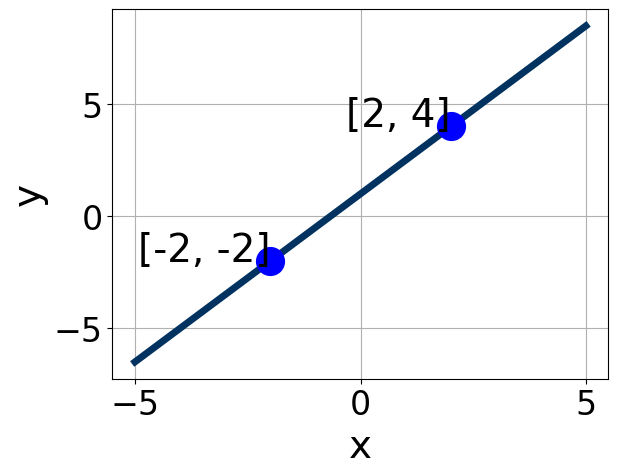
\includegraphics[width=0.5\textwidth]{../Figures/linearGraphToStandardCopyA.png}
\end{center}
\begin{enumerate}[label=\Alph*.]
\item \( A \in [2.84, 4.64], \hspace{3mm} B \in [-2.32, -1.44], \text{ and } \hspace{3mm} C \in [-2.02, -1.52] \)
\item \( A \in [-4.01, -2.79], \hspace{3mm} B \in [1.7, 2.01], \text{ and } \hspace{3mm} C \in [1.22, 3.88] \)
\item \( A \in [2.84, 4.64], \hspace{3mm} B \in [1.7, 2.01], \text{ and } \hspace{3mm} C \in [1.22, 3.88] \)
\item \( A \in [-2.92, -1.26], \hspace{3mm} B \in [0.95, 1.02], \text{ and } \hspace{3mm} C \in [0.78, 1.69] \)
\item \( A \in [-2.92, -1.26], \hspace{3mm} B \in [-1.83, -0.44], \text{ and } \hspace{3mm} C \in [-1.05, -0.64] \)

\end{enumerate} }
\litem{
Solve the equation below. Then, choose the interval that contains the solution.\[ -10(12x + 9) = -18(-19x + 17) \]\begin{enumerate}[label=\Alph*.]
\item \( x \in [-1.03, -0.42] \)
\item \( x \in [0.43, 0.78] \)
\item \( x \in [1.1, 2.23] \)
\item \( x \in [0.6, 1.61] \)
\item \( \text{There are no real solutions.} \)

\end{enumerate} }
\litem{
First, find the equation of the line containing the two points below. Then, write the equation in the form $ y=mx+b $ and choose the intervals that contain $m$ and $b$.\[ (11, -5) \text{ and } (-3, 11) \]\begin{enumerate}[label=\Alph*.]
\item \( m \in [0.14, 4.14] \hspace*{3mm} b \in [14.22, 14.87] \)
\item \( m \in [-3.14, 0.86] \hspace*{3mm} b \in [-16.3, -15.83] \)
\item \( m \in [-3.14, 0.86] \hspace*{3mm} b \in [13.94, 14.32] \)
\item \( m \in [-3.14, 0.86] \hspace*{3mm} b \in [-7.96, -7.54] \)
\item \( m \in [-3.14, 0.86] \hspace*{3mm} b \in [7.19, 8.06] \)

\end{enumerate} }
\litem{
Write the equation of the line in the graph below in Standard Form $Ax+By=C$. Then, choose the intervals that contain $A, B, \text{ and } C$.
\begin{center}
    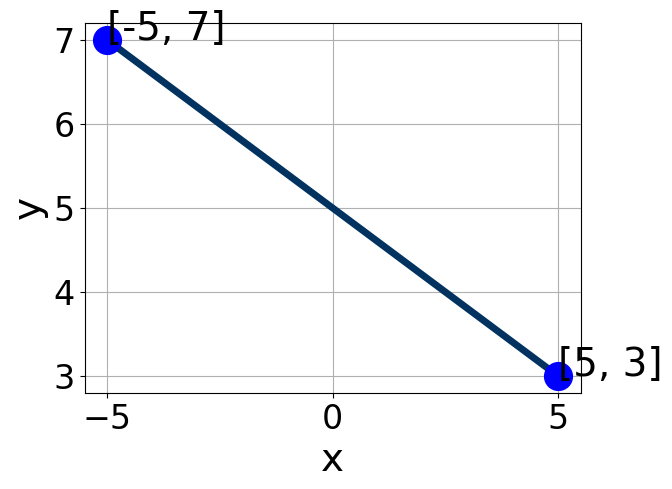
\includegraphics[width=0.5\textwidth]{../Figures/linearGraphToStandardA.png}
\end{center}
\begin{enumerate}[label=\Alph*.]
\item \( A \in [-1.7, 0.9], \hspace{3mm} B \in [-2.32, -0.17], \text{ and } \hspace{3mm} C \in [-7, -3] \)
\item \( A \in [1.6, 3.1], \hspace{3mm} B \in [-7.51, -4.95], \text{ and } \hspace{3mm} C \in [-29, -23] \)
\item \( A \in [-1.7, 0.9], \hspace{3mm} B \in [0.43, 2.07], \text{ and } \hspace{3mm} C \in [1, 12] \)
\item \( A \in [1.6, 3.1], \hspace{3mm} B \in [4.1, 5.67], \text{ and } \hspace{3mm} C \in [24, 31] \)
\item \( A \in [-2.6, 0.2], \hspace{3mm} B \in [-7.51, -4.95], \text{ and } \hspace{3mm} C \in [-29, -23] \)

\end{enumerate} }
\litem{
Solve the equation below. Then, choose the interval that contains the solution.\[ -12(11x -16) = -8(-14x -6) \]\begin{enumerate}[label=\Alph*.]
\item \( x \in [-0.09, 0.98] \)
\item \( x \in [0.87, 0.99] \)
\item \( x \in [11.94, 12.19] \)
\item \( x \in [-1.3, -0.55] \)
\item \( \text{There are no real solutions.} \)

\end{enumerate} }
\litem{
Solve the linear equation below. Then, choose the interval that contains the solution.\[ \frac{4x + 5}{5} - \frac{-3x -8}{2} = \frac{-7x + 3}{8} \]\begin{enumerate}[label=\Alph*.]
\item \( x \in [-0.38, 0.07] \)
\item \( x \in [-4.29, -2.18] \)
\item \( x \in [-2.82, -1.42] \)
\item \( x \in [0.98, 1.57] \)
\item \( \text{There are no real solutions.} \)

\end{enumerate} }
\litem{
Find the equation of the line described below. Write the linear equation in the form $ y=mx+b $ and choose the intervals that contain $m$ and $b$.\[ \text{Perpendicular to } 8 x - 9 y = 9 \text{ and passing through the point } (-9, 4). \]\begin{enumerate}[label=\Alph*.]
\item \( m \in [-1.33, -0.98] \hspace*{3mm} b \in [5.49, 6.27] \)
\item \( m \in [-0.99, -0.73] \hspace*{3mm} b \in [-6.39, -4.95] \)
\item \( m \in [-1.33, -0.98] \hspace*{3mm} b \in [12.5, 13.4] \)
\item \( m \in [0.85, 1.49] \hspace*{3mm} b \in [13.67, 14.79] \)
\item \( m \in [-1.33, -0.98] \hspace*{3mm} b \in [-6.39, -4.95] \)

\end{enumerate} }
\litem{
Solve the linear equation below. Then, choose the interval that contains the solution.\[ \frac{4x + 5}{7} - \frac{8x + 7}{5} = \frac{-3x + 6}{4} \]\begin{enumerate}[label=\Alph*.]
\item \( x \in [-3.19, -1.19] \)
\item \( x \in [1.21, 3.21] \)
\item \( x \in [-9.85, -4.85] \)
\item \( x \in [-30.72, -27.72] \)
\item \( \text{There are no real solutions.} \)

\end{enumerate} }
\litem{
Find the equation of the line described below. Write the linear equation in the form $ y=mx+b $ and choose the intervals that contain $m$ and $b$.\[ \text{Parallel to } 8 x - 9 y = 15 \text{ and passing through the point } (4, 9). \]\begin{enumerate}[label=\Alph*.]
\item \( m \in [0.72, 0.92] \hspace*{3mm} b \in [-8.4, -4] \)
\item \( m \in [1.09, 1.37] \hspace*{3mm} b \in [5.2, 5.7] \)
\item \( m \in [0.72, 0.92] \hspace*{3mm} b \in [5.2, 5.7] \)
\item \( m \in [-0.94, -0.66] \hspace*{3mm} b \in [11.2, 13.6] \)
\item \( m \in [0.72, 0.92] \hspace*{3mm} b \in [2.2, 5.3] \)

\end{enumerate} }
\litem{
First, find the equation of the line containing the two points below. Then, write the equation in the form $ y=mx+b $ and choose the intervals that contain $m$ and $b$.\[ (5, -9) \text{ and } (-3, 11) \]\begin{enumerate}[label=\Alph*.]
\item \( m \in [-5.5, 1.5] \hspace*{3mm} b \in [-4.5, 2.5] \)
\item \( m \in [-5.5, 1.5] \hspace*{3mm} b \in [-15, -13] \)
\item \( m \in [-5.5, 1.5] \hspace*{3mm} b \in [2.5, 4.5] \)
\item \( m \in [1.5, 6.5] \hspace*{3mm} b \in [14.5, 23.5] \)
\item \( m \in [-5.5, 1.5] \hspace*{3mm} b \in [14, 16] \)

\end{enumerate} }
\litem{
Write the equation of the line in the graph below in Standard Form $Ax+By=C$. Then, choose the intervals that contain $A, B, \text{ and } C$.
\begin{center}
    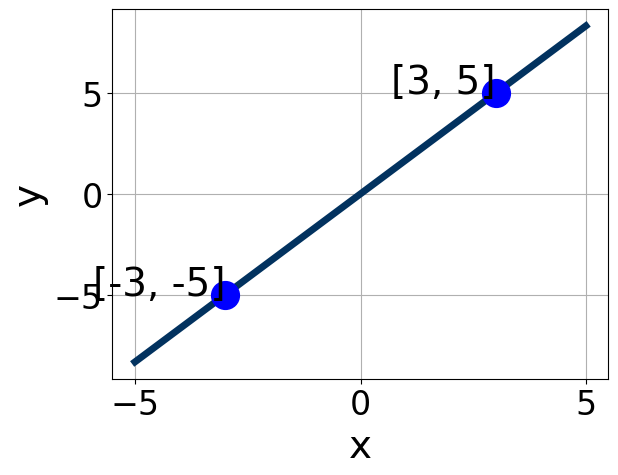
\includegraphics[width=0.5\textwidth]{../Figures/linearGraphToStandardCopyB.png}
\end{center}
\begin{enumerate}[label=\Alph*.]
\item \( A \in [-6, -2], \hspace{3mm} B \in [2, 3.6], \text{ and } \hspace{3mm} C \in [-2, 3] \)
\item \( A \in [-1.67, 2.33], \hspace{3mm} B \in [-1.5, -0.4], \text{ and } \hspace{3mm} C \in [-2, 3] \)
\item \( A \in [-1.67, 2.33], \hspace{3mm} B \in [0, 2.7], \text{ and } \hspace{3mm} C \in [-2, 3] \)
\item \( A \in [4, 7], \hspace{3mm} B \in [-3.9, -2.5], \text{ and } \hspace{3mm} C \in [-2, 3] \)
\item \( A \in [4, 7], \hspace{3mm} B \in [2, 3.6], \text{ and } \hspace{3mm} C \in [-2, 3] \)

\end{enumerate} }
\litem{
Solve the equation below. Then, choose the interval that contains the solution.\[ -8(-2x -18) = -19(-9x + 12) \]\begin{enumerate}[label=\Alph*.]
\item \( x \in [0.54, 0.65] \)
\item \( x \in [2.15, 2.72] \)
\item \( x \in [-0.7, -0.54] \)
\item \( x \in [0.23, 0.52] \)
\item \( \text{There are no real solutions.} \)

\end{enumerate} }
\litem{
First, find the equation of the line containing the two points below. Then, write the equation in the form $ y=mx+b $ and choose the intervals that contain $m$ and $b$.\[ (-8, 5) \text{ and } (6, -3) \]\begin{enumerate}[label=\Alph*.]
\item \( m \in [-1.48, 0.27] \hspace*{3mm} b \in [12.66, 13.75] \)
\item \( m \in [0.51, 0.74] \hspace*{3mm} b \in [-7.37, -5.63] \)
\item \( m \in [-1.48, 0.27] \hspace*{3mm} b \in [-0.63, 0.31] \)
\item \( m \in [-1.48, 0.27] \hspace*{3mm} b \in [0.36, 0.67] \)
\item \( m \in [-1.48, 0.27] \hspace*{3mm} b \in [-9.97, -8.7] \)

\end{enumerate} }
\litem{
Write the equation of the line in the graph below in Standard Form $Ax+By=C$. Then, choose the intervals that contain $A, B, \text{ and } C$.
\begin{center}
    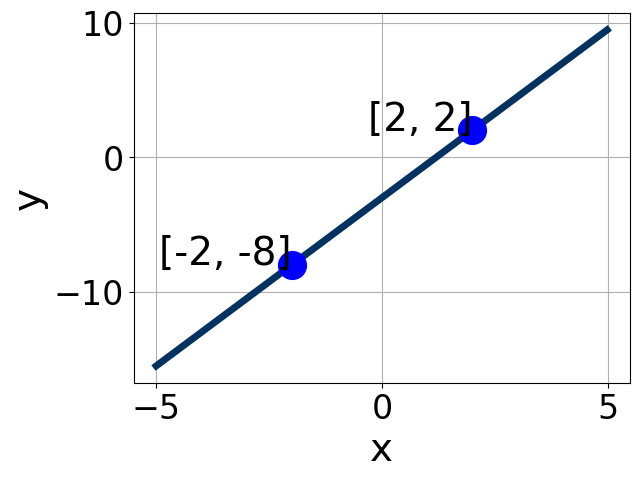
\includegraphics[width=0.5\textwidth]{../Figures/linearGraphToStandardB.png}
\end{center}
\begin{enumerate}[label=\Alph*.]
\item \( A \in [-2.6, 1.8], \hspace{3mm} B \in [-1.74, -0.89], \text{ and } \hspace{3mm} C \in [1.8, 4] \)
\item \( A \in [2.5, 8.3], \hspace{3mm} B \in [1.11, 2.52], \text{ and } \hspace{3mm} C \in [-7.9, -4.8] \)
\item \( A \in [2.5, 8.3], \hspace{3mm} B \in [-2.09, -1.79], \text{ and } \hspace{3mm} C \in [4.8, 8] \)
\item \( A \in [-5.1, -3.2], \hspace{3mm} B \in [1.11, 2.52], \text{ and } \hspace{3mm} C \in [-7.9, -4.8] \)
\item \( A \in [-2.6, 1.8], \hspace{3mm} B \in [-0.04, 1.53], \text{ and } \hspace{3mm} C \in [-5.2, -2.6] \)

\end{enumerate} }
\litem{
Solve the equation below. Then, choose the interval that contains the solution.\[ -14(-15x -6) = -3(18x -12) \]\begin{enumerate}[label=\Alph*.]
\item \( x \in [0.31, 0.74] \)
\item \( x \in [-1.04, -0.76] \)
\item \( x \in [-0.27, -0.14] \)
\item \( x \in [-0.53, -0.33] \)
\item \( \text{There are no real solutions.} \)

\end{enumerate} }
\litem{
Solve the linear equation below. Then, choose the interval that contains the solution.\[ \frac{-3x + 8}{2} - \frac{-8x -7}{3} = \frac{9x + 6}{4} \]\begin{enumerate}[label=\Alph*.]
\item \( x \in [7.9, 9] \)
\item \( x \in [4.4, 5.4] \)
\item \( x \in [0.6, 2] \)
\item \( x \in [0, 0.4] \)
\item \( \text{There are no real solutions.} \)

\end{enumerate} }
\litem{
Find the equation of the line described below. Write the linear equation in the form $ y=mx+b $ and choose the intervals that contain $m$ and $b$.\[ \text{Parallel to } 6 x + 7 y = 12 \text{ and passing through the point } (10, -4). \]\begin{enumerate}[label=\Alph*.]
\item \( m \in [0.16, 1.19] \hspace*{3mm} b \in [-13.13, -12.4] \)
\item \( m \in [-1.07, -0.35] \hspace*{3mm} b \in [2.89, 5.54] \)
\item \( m \in [-1.07, -0.35] \hspace*{3mm} b \in [-6.03, -3.72] \)
\item \( m \in [-1.26, -1.1] \hspace*{3mm} b \in [2.89, 5.54] \)
\item \( m \in [-1.07, -0.35] \hspace*{3mm} b \in [-14.4, -13.93] \)

\end{enumerate} }
\litem{
Solve the linear equation below. Then, choose the interval that contains the solution.\[ \frac{4x + 9}{3} - \frac{4x -4}{7} = \frac{9x + 6}{8} \]\begin{enumerate}[label=\Alph*.]
\item \( x \in [4.62, 5.62] \)
\item \( x \in [18.28, 21.28] \)
\item \( x \in [-1.69, 2.31] \)
\item \( x \in [4.77, 8.77] \)
\item \( \text{There are no real solutions.} \)

\end{enumerate} }
\litem{
Find the equation of the line described below. Write the linear equation in the form $ y=mx+b $ and choose the intervals that contain $m$ and $b$.\[ \text{Perpendicular to } 5 x - 7 y = 7 \text{ and passing through the point } (6, 10). \]\begin{enumerate}[label=\Alph*.]
\item \( m \in [-2.2, -1.21] \hspace*{3mm} b \in [3, 8] \)
\item \( m \in [-1.13, -0.18] \hspace*{3mm} b \in [18.4, 19.4] \)
\item \( m \in [1.05, 1.97] \hspace*{3mm} b \in [0.6, 2.6] \)
\item \( m \in [-2.2, -1.21] \hspace*{3mm} b \in [18.4, 19.4] \)
\item \( m \in [-2.2, -1.21] \hspace*{3mm} b \in [-21.4, -16.4] \)

\end{enumerate} }
\litem{
First, find the equation of the line containing the two points below. Then, write the equation in the form $ y=mx+b $ and choose the intervals that contain $m$ and $b$.\[ (-9, 6) \text{ and } (-8, 10) \]\begin{enumerate}[label=\Alph*.]
\item \( m \in [3, 9] \hspace*{3mm} b \in [14, 16] \)
\item \( m \in [3, 9] \hspace*{3mm} b \in [-42, -40] \)
\item \( m \in [-9, 3] \hspace*{3mm} b \in [-24, -18] \)
\item \( m \in [3, 9] \hspace*{3mm} b \in [39, 43] \)
\item \( m \in [3, 9] \hspace*{3mm} b \in [16, 22] \)

\end{enumerate} }
\litem{
Write the equation of the line in the graph below in Standard Form $Ax+By=C$. Then, choose the intervals that contain $A, B, \text{ and } C$.
\begin{center}
    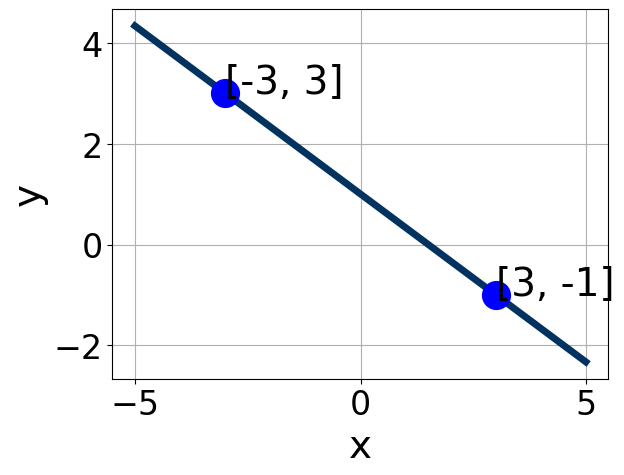
\includegraphics[width=0.5\textwidth]{../Figures/linearGraphToStandardCopyC.png}
\end{center}
\begin{enumerate}[label=\Alph*.]
\item \( A \in [0.9, 2.82], \hspace{3mm} B \in [2.1, 3.2], \text{ and } \hspace{3mm} C \in [2.9, 4.18] \)
\item \( A \in [-0.75, 0.8], \hspace{3mm} B \in [-0.9, 2.3], \text{ and } \hspace{3mm} C \in [0.89, 1.33] \)
\item \( A \in [-0.75, 0.8], \hspace{3mm} B \in [-1.2, 0.9], \text{ and } \hspace{3mm} C \in [-1.63, -0.12] \)
\item \( A \in [0.9, 2.82], \hspace{3mm} B \in [-4.5, -2.4], \text{ and } \hspace{3mm} C \in [-3.28, -2.97] \)
\item \( A \in [-3.19, -0.91], \hspace{3mm} B \in [-4.5, -2.4], \text{ and } \hspace{3mm} C \in [-3.28, -2.97] \)

\end{enumerate} }
\litem{
Solve the equation below. Then, choose the interval that contains the solution.\[ -12(7x -2) = -6(-14x + 16) \]\begin{enumerate}[label=\Alph*.]
\item \( x \in [-0.59, -0.33] \)
\item \( x \in [0.38, 0.58] \)
\item \( x \in [0.67, 0.89] \)
\item \( x \in [-0.24, 0] \)
\item \( \text{There are no real solutions.} \)

\end{enumerate} }
\litem{
First, find the equation of the line containing the two points below. Then, write the equation in the form $ y=mx+b $ and choose the intervals that contain $m$ and $b$.\[ (-9, -5) \text{ and } (-10, -7) \]\begin{enumerate}[label=\Alph*.]
\item \( m \in [1.7, 4.1] \hspace*{3mm} b \in [11.7, 15.01] \)
\item \( m \in [1.7, 4.1] \hspace*{3mm} b \in [3.34, 5.29] \)
\item \( m \in [1.7, 4.1] \hspace*{3mm} b \in [-13.21, -12.4] \)
\item \( m \in [-3, -1.1] \hspace*{3mm} b \in [-28.17, -26.87] \)
\item \( m \in [1.7, 4.1] \hspace*{3mm} b \in [1.52, 3.14] \)

\end{enumerate} }
\litem{
Write the equation of the line in the graph below in Standard Form $Ax+By=C$. Then, choose the intervals that contain $A, B, \text{ and } C$.
\begin{center}
    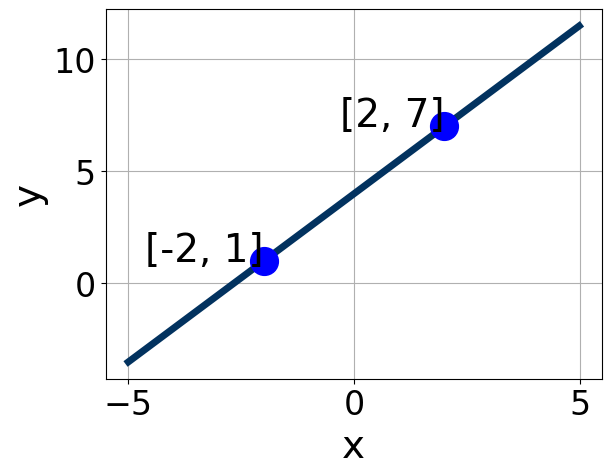
\includegraphics[width=0.5\textwidth]{../Figures/linearGraphToStandardC.png}
\end{center}
\begin{enumerate}[label=\Alph*.]
\item \( A \in [-2.07, -1.15], \hspace{3mm} B \in [-1.44, -0.95], \text{ and } \hspace{3mm} C \in [-5.5, -3.4] \)
\item \( A \in [-3.29, -2.8], \hspace{3mm} B \in [1.96, 2.69], \text{ and } \hspace{3mm} C \in [7.3, 10.1] \)
\item \( A \in [1.55, 3.68], \hspace{3mm} B \in [1.96, 2.69], \text{ and } \hspace{3mm} C \in [7.3, 10.1] \)
\item \( A \in [1.55, 3.68], \hspace{3mm} B \in [-2.26, -1.9], \text{ and } \hspace{3mm} C \in [-8.9, -7.4] \)
\item \( A \in [-2.07, -1.15], \hspace{3mm} B \in [0.54, 1.34], \text{ and } \hspace{3mm} C \in [3.4, 5.6] \)

\end{enumerate} }
\litem{
Solve the equation below. Then, choose the interval that contains the solution.\[ -15(8x + 3) = -9(14x -6) \]\begin{enumerate}[label=\Alph*.]
\item \( x \in [-2.8, -0.5] \)
\item \( x \in [-1.2, 0.1] \)
\item \( x \in [0.5, 2.6] \)
\item \( x \in [15.7, 17.6] \)
\item \( \text{There are no real solutions.} \)

\end{enumerate} }
\litem{
Solve the linear equation below. Then, choose the interval that contains the solution.\[ \frac{-4x + 7}{8} - \frac{7x + 3}{5} = \frac{-6x -3}{4} \]\begin{enumerate}[label=\Alph*.]
\item \( x \in [16.5, 19.5] \)
\item \( x \in [0.2, 2.2] \)
\item \( x \in [5.56, 8.56] \)
\item \( x \in [1.56, 4.56] \)
\item \( \text{There are no real solutions.} \)

\end{enumerate} }
\litem{
Find the equation of the line described below. Write the linear equation in the form $ y=mx+b $ and choose the intervals that contain $m$ and $b$.\[ \text{Parallel to } 5 x - 8 y = 12 \text{ and passing through the point } (-4, -3). \]\begin{enumerate}[label=\Alph*.]
\item \( m \in [0.74, 3.04] \hspace*{3mm} b \in [-1.67, 0.09] \)
\item \( m \in [-0.16, 0.63] \hspace*{3mm} b \in [0.59, 1.56] \)
\item \( m \in [-2.11, -0.52] \hspace*{3mm} b \in [-5.65, -5.1] \)
\item \( m \in [-0.16, 0.63] \hspace*{3mm} b \in [-0.06, 0.58] \)
\item \( m \in [-0.16, 0.63] \hspace*{3mm} b \in [-1.67, 0.09] \)

\end{enumerate} }
\litem{
Solve the linear equation below. Then, choose the interval that contains the solution.\[ \frac{6x -7}{7} - \frac{-3x + 9}{5} = \frac{3x -3}{8} \]\begin{enumerate}[label=\Alph*.]
\item \( x \in [11.3, 13.9] \)
\item \( x \in [-0.4, 2] \)
\item \( x \in [2, 2.9] \)
\item \( x \in [-1.2, -0.9] \)
\item \( \text{There are no real solutions.} \)

\end{enumerate} }
\litem{
Find the equation of the line described below. Write the linear equation in the form $ y=mx+b $ and choose the intervals that contain $m$ and $b$.\[ \text{Perpendicular to } 7 x - 4 y = 8 \text{ and passing through the point } (-3, 2). \]\begin{enumerate}[label=\Alph*.]
\item \( m \in [-0.5, 0.9] \hspace*{3mm} b \in [3.52, 4.84] \)
\item \( m \in [-1.11, 0.04] \hspace*{3mm} b \in [4.56, 5.52] \)
\item \( m \in [-2.96, -0.9] \hspace*{3mm} b \in [0.2, 0.5] \)
\item \( m \in [-1.11, 0.04] \hspace*{3mm} b \in [-0.97, 0.16] \)
\item \( m \in [-1.11, 0.04] \hspace*{3mm} b \in [0.2, 0.5] \)

\end{enumerate} }
\end{enumerate}

\end{document}